\documentclass[12pt, a4paper]{article}
\usepackage[utf8]{inputenc}
\usepackage[russian,english]{babel}
\usepackage[T2A]{fontenc}
\usepackage[left=10mm, top=20mm, right=18mm, bottom=15mm, footskip=10mm]{geometry}
\usepackage{indentfirst}
\usepackage{amsmath,amssymb}
\usepackage[italicdiff]{physics}
\usepackage{graphicx}
\graphicspath{{images/}}
\DeclareGraphicsExtensions{.pdf,.png,.jpg}
\usepackage{wrapfig}
\usepackage{float}
\usepackage{subcaption}
\usepackage{enumitem}
\usepackage{caption}
\usepackage{array}
\usepackage[russian]{babel}
\usepackage{ragged2e}
\captionsetup[figure]{name=Рисунок}
\captionsetup[table]{name=Таблица}

\renewcommand{\contentsname}{Содержание}

\begin{document}

% Оглавление без надписи
\tableofcontents
\newpage

\section{Введение}
\begin{justify}
Уникальной и перспективной технологией для измерения параметров движения и волновых полей являются системы, построенные на основе явления конвективной диффузии в растворах электролитов. Они не содержат элементов точной механики, а в качестве инерционной массы и преобразующего элемента внешнего воздействия в электрический ток используется жидкость, которая, подобно <<электронному газу>> в вакуумных приборах, осуществляет перенос активных носителей заряда, 
промодулированный внешним механическим сигналом. Основная физическая идея подобного устройства позаимствована из вакуумной электроники. В самом деле, увеличение тока в вакуумном триоде можно осуществить не только изменением сеточного напряжения, но также и простым перемещением сетки, например под действием внешнего механического сигнала.
\par
В то время как создать подобный преобразователь механического 
воздействия на базе вакуумного триода технически крайне сложно, данная идея осуществима в системах на основе проводящей жидкости. 
\par
Если на электроды подана разность потенциалов, то между анодом и катодом устанавливается стационарное распределение концентрации активных носителей заряда, ведущее к возникновению постоянного электрического тока, пропорционального градиенту концентрации на электродах. При воздействии внешнего сигнала происходит перемещение рабочей жидкости и увлечение ею активных ионов, которое ведет к изменению их концентрации на электродах. Соответственно во внешней цепи происходят вариации тока. При этом подобно тому, как это происходит в вакуумном триоде, осуществляется усиление сигнала по мощности за счет использования энергии внешнего источника. Коэффициент преобразования механического возмущения в электрический ток при этом достигает $1\,\frac{\text{А}}{\text{м/с}}$, что существенно превышает чувствительность электродинамических систем, широко распространенных в сейсмологии в настоящее время, и делает электрохимические преобразователи пригодными для регистрации удаленных землетрясений и прочих колебаний малой амплитуды.
\end{justify}
\begin{figure}[!hb]
	\centering
	
\includegraphics[width=0.9\linewidth]{p1.png}
	\caption{Молекулярно-электронный преобразователь }
	\label{pic_3}
\end{figure}

\newpage
Наибольшее распространение получили молекулярно-электронные преобразователи (МЭП), выполненные на базе двух электрохимических ячеек (ЭЯ), включенных по дифференциальной схеме. Принципиальная схема такого преобразователя показана на рис. 1. 

Конструкция устройства включает следующие основные элементы:
\begin{itemize}[label=--]
    \item \textbf{Диэлектрическая трубка} (1);
    \item \textbf{Электродный узел} (2), помещенный внутрь трубки;
    \item \textbf{Раствор электролита} (3), заполняющий внутренний объем;
    \item \textbf{Плоские сетчатые электроды}, установленные внутри узла:
    \begin{itemize}
        \item аноды (5);
        \item катоды (6);
    \end{itemize}
    \item \textbf{Пористые перегородки} (4), разделяющие электроды.
\end{itemize}
В МЭП могут быть использованы различные окислительно-восстановительные реакции, например: йод - йодид, ферро - феррицианид и др. При этом чаще всего электроды ЭЯ изготавливаются из металла, который не участвует в обмене катионами, а осуществляет только электронный обмен.

В настоящее время наиболее широкое применение получили йод-йодидные системы с платиновыми электродами [1, 4]. Электролит такой системы состоит из водного раствора йодида калия $KI$ и йода $I_2$. В избытке йодида йод переходит в хорошо растворимое комплексное соединение - трийодид по следующей схеме:
\[
I_2 + I^- \rightarrow I_3^-.
\]
При прохождении тока через МЭЯ на катодах происходит восстановление йода:
\[
I_3^- + 2e \rightarrow 3I^-;
\]
а на аноде окисление йода:
\[
3I^- - 2e \rightarrow I_3^-.
\]
Ионы калия не принимают участия в реакциях.
\par

Электрический ток, проходящий через ЭЯ, определяется как концентрацией ионов, так и механизмом их движения в растворах электролитов. Перенос заряда в жидкости можно разделить на три независимых механизма: миграция, диффузия и конвекция, каждый из них в определенных физико-химических процессах играет главную роль.

\par

Математическая формулировка задачи для расчета тока, текущего через электрохимическую ячейку, сводится к решению уравнений гидродинамики и диффузии:
\begin{align}
    \frac{\partial \mathbf{v}}{\partial t} + (\mathbf{v}\nabla)\mathbf{v} &= -\frac{\nabla p}{\rho} + \gamma\Delta\mathbf{v} + \label{eq:1} \\
    \operatorname{div} \mathbf{v} &= 0 \label{eq:2} \\
    \frac{\partial n}{\partial t} &= D\Delta n + (\mathbf{v}, \nabla)n + \label{eq:3}
\end{align}
где $\mathbf{v}$ -- скорость электролита, $p$ -- давление, $\rho$ -- плотность электролита, $\nu$ -- вязкость жидкости, $n$ -- концентрация носителей тока (ионов трийодида), $D$ -- коэффициент их диффузии, $j$ -- плотность потока. В системе с плоскими электродами эти уравнения фактически являются одномерными.

В качестве граничных условий к уравнениям (3) - (4) используются следующие соотношения:
\begin{enumerate}
    \item Отсутствие потока активных ионов через диэлектрические поверхности.
    \item Уравнения, определяющие скорости электрохимических реакций в зависимости от концентрации ионов и скачка потенциала на границе электрод/электролит. Получение таких уравнений является предметом отдельной области исследований -- электродной кинетики.
\end{enumerate}

Кроме того, дополнительно накладывается интегральное соотношение, выражающее закон сохранения количества активных ионов
\begin{equation}
\iiint n(x, y, z, t) dV = V n_0, \tag{4}
\end{equation}
где $V$ -- объем электролита, $n_0$ -- равновесная концентрация.

Следует отметить, что система уравнений (1) - (3) является приближенной и не учитывает наличие в МЭЯ электрического поля и объемного заряда, которые могут влиять на гидродинамическое движение раствора и конвективный перенос ионов.

Ниже будут рассмотрены решения уравнения (1) -- (3) в некоторых частных случаях, представляющих практический интерес.

\section*{Стационарный случай}

Величина диффузионного тока, текущего через электрод:
\[
I_D = -eSD\nabla n
\]
В стационарном случае уравне
ние диффузии (3) будет иметь вид:
\[
\Delta n = 0.
\]

Выражение для тока, текущего через 
катод или анод: 

\begin{equation}
I_D = -\frac{e S D n_0}{d} \, \mathrm{th}\!\left( \frac{e U}{2 k_\mathrm{B} T} \right).
\label{eq:diode_current}
\end{equation}

Соответствующая вольт-амперная характеристика представлена на 
рис:

\begin{figure}[!hb]
	\centering
	
\includegraphics[width=0.7\linewidth]{p2.png}
	\caption{ВАХ молекулярно-электронной ячейки с неподвижным электролитом }
	\label{pic_3}
\end{figure}
\newpage

\section*{Конвективная диффузия}

Если жидкость в МЭР приходит в движение под действием каких-либо внешних сил, то, наряду с диффузионным, появляется также конвективный ток, обусловленный увлечением ионов движущейся жидкостью. В линейном приближении конвективный ток пропорционален скорости движущейся жидкости $V$ и определяется соотношением:
\begin{equation}
I_k = e S n V.
\label{eq:convective_current}
\end{equation}

Полезно сравнить, при каких минимальных скоростях движения жидкости конвективный ток становится сравнимым с диффузионным. Для оценок положим расстояние между электродами $d \approx 10^{-2}\,\mathrm{см}$, $D = 10^{-5}\,\mathrm{см^2/с}$ получаем $I_D \approx I_k$ при $V \approx 10^{-3}\,\mathrm{см/с}$. Это означает, что столь малое значение скорости движения жидкости способно изменить ток в цепи МЭР на величину, сравнимую с ним самой. Именно этим объясняется высокая чувствительность молекулярно-электронных преобразователей к действию внешних механических возмущений.

В основе работы МЭЯ лежит конвективная диффузия, вызванная действием внешних механических возмущений. 

Найдём изменение тока через молекулярно-электронный преобразователь, вызванное протеканием электролита. В случае малых изменений механических величин можно ограничиться линейным приближением. В этом приближении введём для удобства новую переменную $c(x,t)$, которая определяется из выражения
\begin{equation}
n = n_0 \left( 1 - \frac{x}{d} \, \mathrm{th}\!\left( \frac{eU}{2k_\mathrm{B}T} \right) \right) + c(x,t).
\label{eq:carrier_concentration_perturbation}
\end{equation}

В этом случае уравнение конвективной диффузии перепишем:

\begin{equation}
\frac{\partial c}{\partial t} - D \frac{\partial^2 c}{\partial x^2} = V_0 e^{i\omega t} \, \frac{n_0}{d} \, \mathrm{th}\!\left( \frac{eU}{2k_\mathrm{B}T} \right).
\label{eq:diffusion_perturbation_equation}
\end{equation}

Решение:

\begin{equation}
X(x) = A_1 e^{(1+i)\sqrt{\frac{\omega}{2D}}\,x} + A_2 e^{-(1+i)\sqrt{\frac{\omega}{2D}}\,x} - \frac{i V_0 n_0}{d \omega} \, \mathrm{th}\!\left( \frac{eU}{2k_\mathrm{B}T} \right).
\label{eq:solution_X_x}
\end{equation}

Для определения постоянных воспользуемся граничными условиями и получим:

\begin{equation}
X(d) = X(-d) = 0.
\label{eq:boundary_conditions_X}
\end{equation}

В результате получим:
\begin{equation}
A_1 = A_2 = i \, \frac{V_0 n_0}{2 d \omega} \, \frac{\mathrm{th}\!\left( \dfrac{eU}{2k_\mathrm{B}T} \right)}{\ch\!\left( (1+i)\sqrt{\dfrac{\omega}{2D}}\, d \right)}.
\label{eq:A1_A2_solution}
\end{equation}

Окончательно, для концентрации $c(x,t)$ имеем
\begin{equation}
c(x,t) = i \, \frac{V_0 n_0}{d \omega} \, \mathrm{th}\!\left( \frac{eU}{2k_\mathrm{B}T} \right) e^{i\omega t} \left( \frac{ \ch\!\left( (1+i)\sqrt{\dfrac{\omega}{2D}}\, x \right) }{ \ch\!\left( (1+i)\sqrt{\dfrac{\omega}{2D}}\, d \right) } - 1 \right).
\label{eq:concentration_final}
\end{equation}

Выражение для полного тока, те
кущего через систему:

\begin{equation}
I = -\frac{e S D n_0}{d} \, \mathrm{th}\!\left( \frac{eU}{2k_\mathrm{B}T} \right) \left[ 1 - e^{i\omega t}(1 - i) \sqrt{\frac{1}{2\omega D}} \, V_0 \, t h\!\left( (1 + i) \sqrt{\frac{\omega}{2D}} \, d \right) \right].
\label{eq:current_full_expression}
\end{equation}

\newpage

\begin{figure}[!hb]
	\centering
	
\includegraphics[width=0.8\linewidth]{p3.png}
	\caption{ависимость модуля выходного тока МЭЯ от частоты в условиях 
конвективной диффузии }
	\label{pic_3}
\end{figure}

\section{Цель работы и оборудование}

\textbf{Цель работы}: Исследование процессов протекания тока в молекулярно
-электронном преобразователе в стационарных и нестационарных условиях. 

\textbf{Оборудование и ПО}: Для задания входных сигналов и регистрации  полученных данных 
используется программа calib  управления многофункциональным моду
лем ЦАП/АЦП. Обработка данных осуществляется с помощью пакета Dadisp. 
\newpage
\section{Методика эксперимента}

Для стационарного случая проводится измерение ВАХ, т.е. зависимости выходного тока ЭЯ в условиях стационарной диффузии от приложенной к электродам разности потенциалов.
\par

На рисунке приведена схема устройства:

\begin{figure}[!hb]
	\centering
	
\includegraphics[width=0.8\linewidth]{p4.png}
	\caption{Принципиальная схема экспериментальной установки для измерения стационарной ВАХ}
	\label{pic_3}
\end{figure}

\section{Ход работы}

\begin{table}[h]
\centering
\renewcommand{\arraystretch}{1.5}
\begin{tabular}{|l|c|c|c|c|c|c|c|c|c|c|c|c|c|}
\hline
\textbf{U, мВ} & \textbf{0} & \textbf{2} & \textbf{5} & \textbf{10} & \textbf{15} & \textbf{20} & \textbf{30} & \textbf{40} & \textbf{50} & \textbf{100} & \textbf{150} & \textbf{200} & \textbf{400} \\ \hline
\textbf{U\textsubscript{цп}, мВ} &  &  & -51,7 & -56,7 &  &  &  &  &  &  &  & -247 & -447 \\ \hline
\textbf{U\textsubscript{ацп}, мВ} & -62,9 & -48,8 & -23,1 & 13,4 & 49,3 & 81,9 & 138 & 186 & 230,9 & 427 & 597 & 708 & 954 \\ \hline
\textbf{I, мкА} & -6,29 & -4,88 & -2,31 & 1,34 & 4,93 & 8,19 & 13,8 & 18,6 & 23,09 & 42,7 & 59,7 & 70,8 & 95,4 \\ \hline
\end{tabular}
\caption{Измерение ВАХ}
\label{tab:measurements}
\end{table}

График:
\newpage

\begin{figure}[!hb]
	\centering
	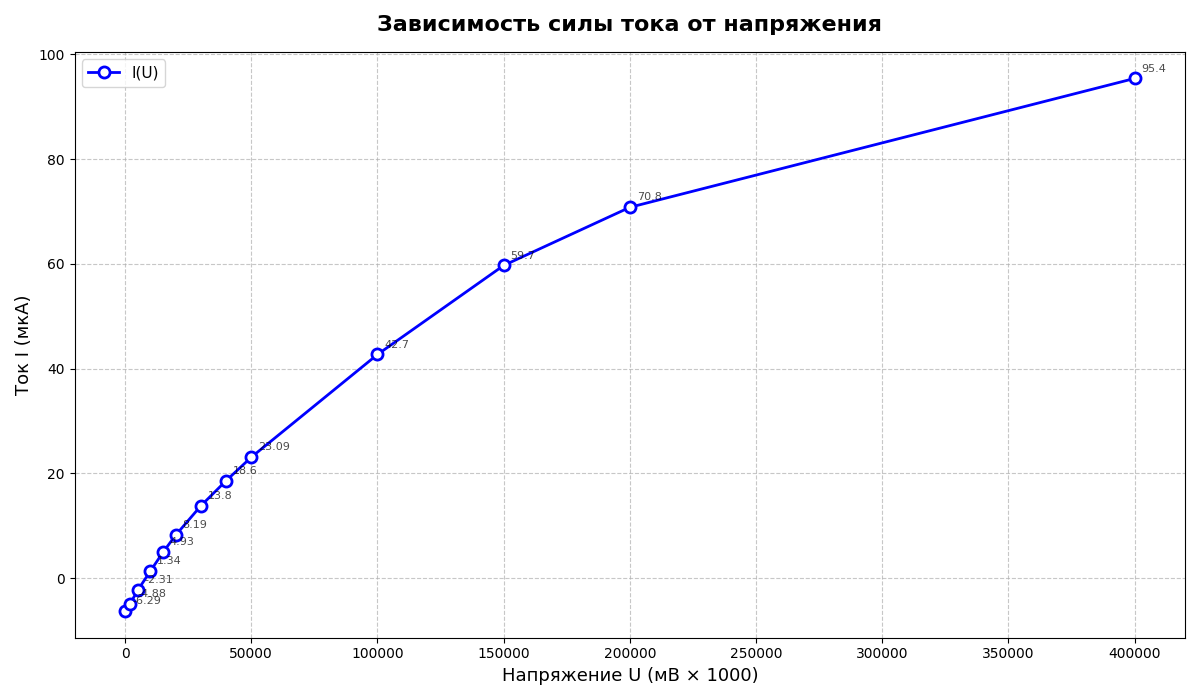
\includegraphics[width=1.1\linewidth]{f1.png}
	\caption{ВАХ}
	\label{pic_3}
\end{figure}

Оценим площадь электродов: 

\begin{equation}
I_0 = \frac{e S D n_0}{d},
\label{eq:steady_current_diffusion}
\end{equation}
откуда
\begin{equation}
S = \frac{I_0 d}{e D n_0}.
\label{eq:area_from_current}
\end{equation}

Все величины подставляем в системе СИ:
\begin{itemize}
    \item $I_0 = 96~\mathrm{мкА} = 96 \times 10^{-6}~\mathrm{А}$;
    \item $d = 50~\mathrm{мкм} = 50 \times 10^{-6}~\mathrm{м}$;
    \item $e = 1.602 \times 10^{-19}~\mathrm{Кл}$;
    \item $D = 10^{-5}~\mathrm{см^2/с} = 10^{-9}~\mathrm{м^2/с}$;
    \item $n_0 = 10^{25}~\mathrm{м^{-3}}$ 
\end{itemize}
Подставив, получим:
\[S = 3,0 \text{мм}^{2}\]

\newpage

Проведем измерение АЧХ:

\begin{table}[h!]
\centering
\renewcommand{\arraystretch}{1.5} % Увеличиваем высоту строк для читаемости
\begin{tabular}{|p{4cm}|c|c|c|c|c|c|c|c|}
\hline
Частота, Гц & 0,1 & 0,2 & 0,5 & 1 & 2 & 5 & 10 & 20 \\ \hline
Размах входного сигнала Uвх, мВ & 49 & 50 & 49 & 50 & 49 & 50 & 49 & 50 \\ \hline
Размах выходного сигнала Uвых, мВ & 151 & 215 & 287 & 264 & 269 & 167 & 76 & 27 \\ \hline
Отношение Uвых/Uвх & 3,08 & 4,3 & 5,9 & 5,28 & 5,48 & 3,34 & 1,55 & 0,54 \\ \hline
\end{tabular}
\end{table}

Графики:

\begin{figure}[!hb]
	\centering
	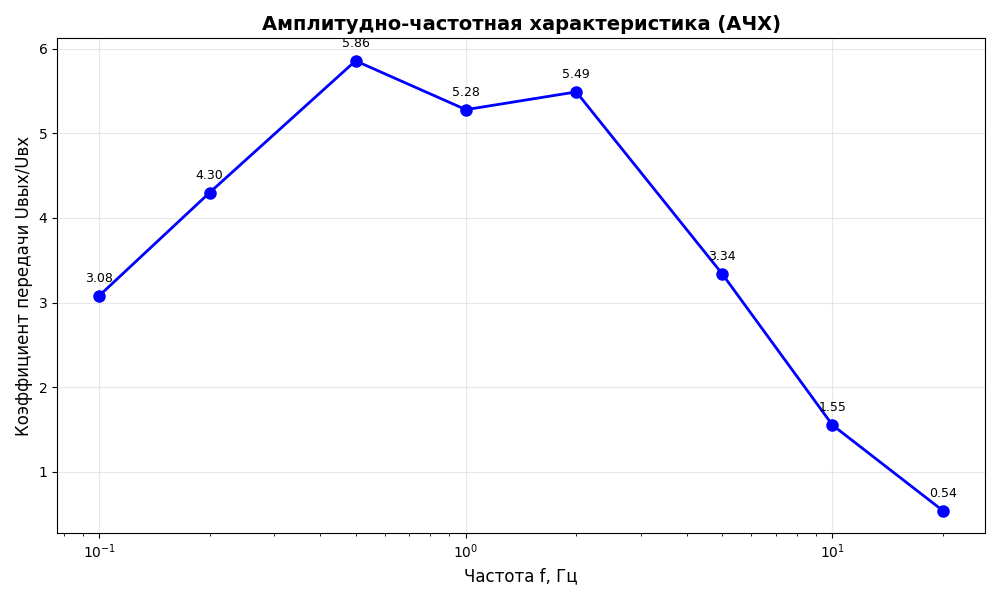
\includegraphics[width=1.1\linewidth]{f2.png}
	\caption{АЧХ}
	\label{pic_3}
\end{figure}

\newpage

\begin{figure}[!hb]
	\centering
	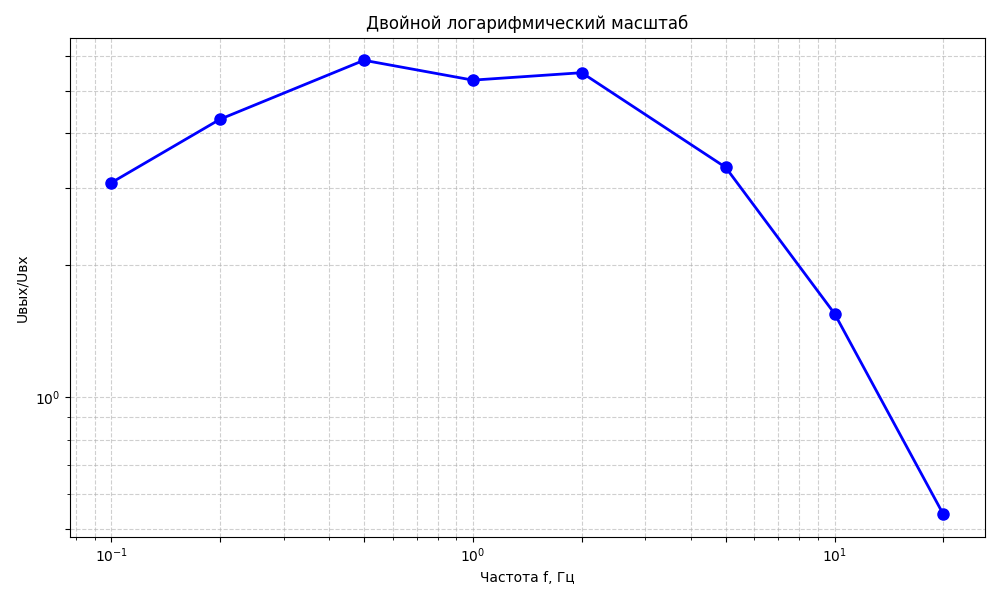
\includegraphics[width=1.1\linewidth]{f3.png}
	\caption{АЧХ в двойном логарифмическом масштабе}
	\label{pic_3}
\end{figure}

\section{Вывод}
Исследовали процессы протекания тока в молекулярно электронном преобразователев стационарных и нестационарных условиях.

\end{document}